\section{Функции обработчика прерывания от системного таймера в защищенном режиме в Windows}

\begin{enumerate}
	\item по тику
	\begin{itemize}
		\item ...
	\end{itemize}
	\item по главному тику
	\begin{itemize}
		\item ...
	\end{itemize}
	\item по кванту
	\begin{itemize}
		\item ...
	\end{itemize}
\end{enumerate}

\section{Функции обработчика прерывания от системного таймера в защищенном режиме в Unix}

\begin{enumerate}
	\item по тику
	\begin{itemize}
		\item ...
	\end{itemize}
	\item по главному тику
	\begin{itemize}
		\item ...
	\end{itemize}
	\item по кванту
	\begin{itemize}
		\item ...
	\end{itemize}
\end{enumerate}




% \begin{figure}[ht!]
% 	\centering{
% 		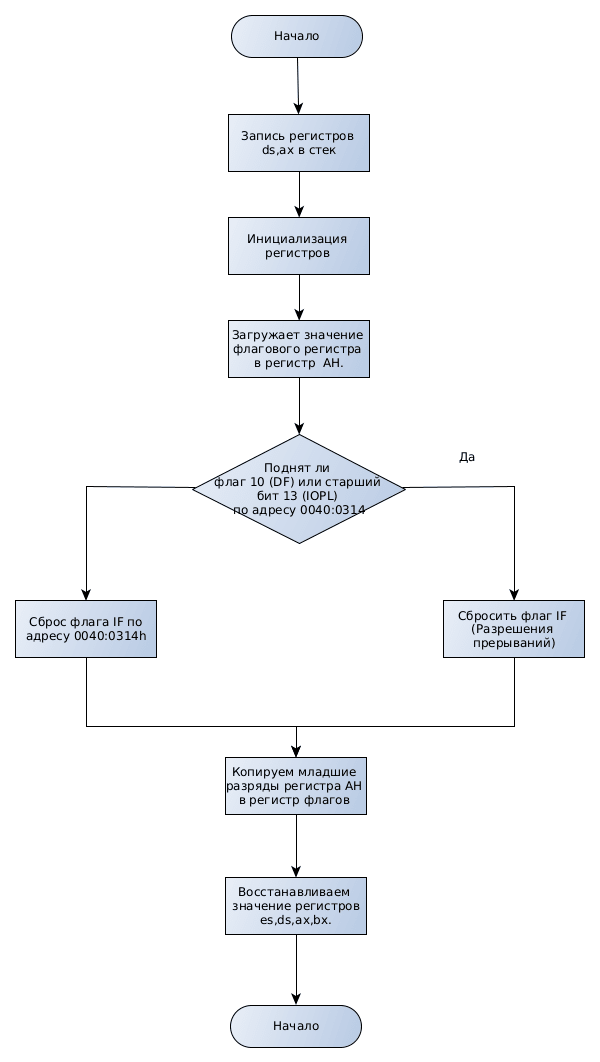
\includegraphics[width=0.6\textwidth]{img/graph3.png}
% 		\caption{Схема подпрограммы sub\_1} }
% \end{figure}